\documentclass[12pt]{article}

\usepackage{amsmath, mathtools}
\usepackage{amsfonts}
\usepackage{amssymb}
\usepackage{graphicx}
\usepackage{colortbl}
\usepackage{xr}
\usepackage{hyperref}
\usepackage{longtable}
\usepackage{xfrac}
\usepackage{tabularx}
\usepackage{float}
\usepackage{siunitx}
\usepackage{booktabs}
\usepackage{caption}
\usepackage{pdflscape}
\usepackage{afterpage}

\usepackage[round]{natbib}

%\usepackage{refcheck}

\hypersetup{
    bookmarks=true,         % show bookmarks bar?
      colorlinks=true,       % false: boxed links; true: colored links
    linkcolor=red,          % color of internal links (change box color with linkbordercolor)
    citecolor=green,        % color of links to bibliography
    filecolor=magenta,      % color of file links
    urlcolor=cyan           % color of external links
}

%% Comments

\usepackage{color}

\newif\ifcomments\commentstrue

\ifcomments
\newcommand{\authornote}[3]{\textcolor{#1}{[#3 ---#2]}}
\newcommand{\todo}[1]{\textcolor{red}{[TODO: #1]}}
\else
\newcommand{\authornote}[3]{}
\newcommand{\todo}[1]{}
\fi

\newcommand{\wss}[1]{\authornote{blue}{SS}{#1}}
\newcommand{\an}[1]{\authornote{magenta}{Author}{#1}}
\newcommand{\wss}[1]{\authornote{blue}{SS}{#1}}



% For easy change of table widths
\newcommand{\colZwidth}{1.0\textwidth}
\newcommand{\colAwidth}{0.13\textwidth}
\newcommand{\colBwidth}{0.82\textwidth}
\newcommand{\colCwidth}{0.1\textwidth}
\newcommand{\colDwidth}{0.05\textwidth}
\newcommand{\colEwidth}{0.8\textwidth}
\newcommand{\colFwidth}{0.17\textwidth}
\newcommand{\colGwidth}{0.5\textwidth}
\newcommand{\colHwidth}{0.28\textwidth}

% Used so that cross-references have a meaningful prefix
\newcounter{defnum} %Definition Number
\newcommand{\dthedefnum}{GD\thedefnum}
\newcommand{\dref}[1]{GD\ref{#1}}
\newcounter{datadefnum} %Datadefinition Number
\newcommand{\ddthedatadefnum}{DD\thedatadefnum}
\newcommand{\ddref}[1]{DD\ref{#1}}
\newcounter{theorynum} %Theory Number
\newcommand{\tthetheorynum}{T\thetheorynum}
\newcommand{\tref}[1]{T\ref{#1}}
\newcounter{tablenum} %Table Number
\newcommand{\tbthetablenum}{T\thetablenum}
\newcommand{\tbref}[1]{TB\ref{#1}}
\newcounter{assumpnum} %Assumption Number
\newcommand{\atheassumpnum}{P\theassumpnum}
\newcommand{\aref}[1]{A\ref{#1}}
\newcounter{goalnum} %Goal Number
\newcommand{\gthegoalnum}{P\thegoalnum}
\newcommand{\gsref}[1]{GS\ref{#1}}
\newcounter{instnum} %Instance Number
\newcommand{\itheinstnum}{IM\theinstnum}
\newcommand{\iref}[1]{IM\ref{#1}}
\newcounter{reqnum} %Requirement Number
\newcommand{\rthereqnum}{P\thereqnum}
\newcommand{\rref}[1]{R\ref{#1}}
\newcounter{lcnum} %Likely change number
\newcommand{\lthelcnum}{LC\thelcnum}
\newcommand{\lcref}[1]{LC\ref{#1}}

\newcommand{\famname}{FFT} % PUT YOUR PROGRAM NAME HERE

\usepackage{fullpage}

\begin{document}

\title{FFT Library} 
\author{Yuzhi Zhao}
\date{\today}
\maketitle


\newpage

\tableofcontents

~\newpage

\pagenumbering{roman}

\section{Revision History}

\begin{tabularx}{\textwidth}{p{3cm}p{2cm}X}
\toprule {\bf Date} & {\bf Version} & {\bf Notes}\\
\midrule
Date 1 & 1.0 & Notes\\
Date 2 & 1.1 & Notes\\
\bottomrule
\end{tabularx}

~\newpage
	
\section{Reference Material}

This section records information for easy reference.

\subsection{Table of Units}

Throughout this document SI (Syst\`{e}me International d'Unit\'{e}s) is employed
as the unit system.  In addition to the basic units, several derived units are
used as described below.  For each unit, the symbol is given followed by a
description of the unit and the SI name.
~\newline

\renewcommand{\arraystretch}{1.2}
%\begin{table}[ht]
  \noindent \begin{tabular}{l l l} 
    \toprule		
    \textbf{symbol} & \textbf{unit} & \textbf{SI}\\
    \midrule 
    \si{\volt} & voltage & volt\\
    \si{\watt} & power & Watt (W = \si{\joule\per\second})\\
    \si{\hertz} &frequency& Hertz\\
    \si{\decibel} & decibel & Decibel\\
    \bottomrule
  \end{tabular}
  %	\caption{Provide a caption}
%\end{table}

  \wss{For an FFT library, you don't really need many units.  You don't know if your
    ``signal'' for the FFT is a voltage, or a current, or stock prices, or
    concentration of CO$_2$ in the atmosphere.  The user of the library will be
    responsible for knowing the meaning of the input.  My initial thinking is
    that the only unit that makes sense for all potential applications is your
    units for frequency.}

\subsection{Table of Symbols}

The table that follows summarizes the symbols used in this document along with
their units.  The choice of symbols was made to be consistent with the heat
transfer literature and with existing documentation for solar water heating
systems.  The symbols are listed in alphabetical order.

\renewcommand{\arraystretch}{1.2}
%\noindent \begin{tabularx}{1.0\textwidth}{l l X}
\noindent \begin{longtable*}{l l p{12cm}} \toprule
\textbf{symbol} & \textbf{unit} & \textbf{description}\\
\midrule 
$a_n$ & none & coefficient of real number
\\
$b_n$ &none &coefficient of complex number
\\ 
\bottomrule
\end{longtable*}

\wss{You do not have all of your symbols in this list.}

\subsection{Abbreviations and Acronyms}

\renewcommand{\arraystretch}{1.2}
\begin{tabular}{l l} 
  \toprule		
  \textbf{symbol} & \textbf{description}\\
  \midrule 
  A & Assumption\\
  DD & Data Definition\\
  GS & Goal Statement\\
  IM & Instance Model\\
  SRS & Software Requirements Specification\\
  \famname{} & Fast Fourier Transform\\
  T & Theoretical Model\\
  DFT & Discrete Fourier Transform\\
  IDFT & Invers Discrete Transform\\
  \bottomrule
\end{tabular}\\

\pagenumbering{arabic}

\section{Introduction}

Fast Fourier transforms are widely used for many applications in engineering, science, and mathematics. FFT's importance derives from the fact that in signal processing and image processing it has made working in frequency domain equally computationally feasible as working in temporal or spatial domain. \\

\wss{The text is better for version control, and for reading in other editors,
  if you use a hard-wrap at 80 characters}

The following section provides an overview of the Software Requirements
Specification (SRS) for a FFT Library.  The
developed program will be referred to as Fast Fourier Transform Library
(\famname{}).  This section explains the purpose of this document, the scope of
the system, the characteristics of the intended readers and the organization of
the document.

\subsection{Purpose of Document}

This document will be  used as a starting point for subsequent development phases, including writing the design specification and the software verification and validation plan.
The design document will show how the requirements are to be realized, including decisions on the numerical algorithms and programming environment.
The verification and validation plan will show the steps that will be used to increase confidence in the software documentation and the implementation.

\subsection{Scope of the Family} 

The scope of the requirements includes specifing \wss{spell check!} the input
data, specifying the number of radix of FFT. Given the full information of input
and parameters, the FFT Library will take advantage of FFT algorithms to do DFT
or IDFT calcualtion \wss{spell check!} effectively.

\subsection{Characteristics of Intended Reader} 

Reviewers of this documentation should have a strong knowledge in Complex
Variables Functions as well as have an understanding of differential
equaltions. \wss{spell check!} \wss{For the characteristics of intended reader
  try to be more specific about the education.  What degree?  What course areas?
  What level?}

\subsection{Organization of Document}
The organization of this document follows the template for an SRS for scientific
computing software proposed by~\cite{Koothoor2013} \wss{missing citation in your
  bib file} and \cite{SmithAndLai2005}.
The presentation follows the standard pattern of presenting goals, theories,
definitions, and assumptions.  For readers that would like a more bottom up
approach, they can start reading the instance models in Section
\ref{sec_instance} and trace back to find any additional information they
require.  The instance models provide the algebraic equations that model the FFT algorithm.


\section{General System Description}

This section identifies the interfaces between the system and its environment,
describes the potential user characteristics and lists the potential system
constraints.

\subsection{Potential System Contexts}

Figure~\ref{Fig_SystemContext} shows the system context.  A circle represents an
external entity outside the software, the user in this case.  A rectangle
represents the software system itself (\famname{}).  Arrows are used to show the data
flow between the system and its environment.

\wss{You should clarify that the user could be a program that is using your library.}

\begin{figure}[h!]
\begin{center}
 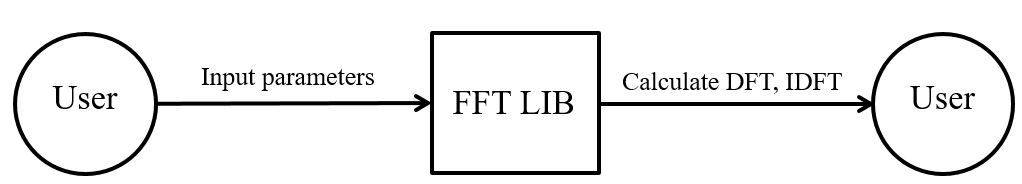
\includegraphics[width=0.6\textwidth]{SystemContextFigure}
\caption{System Context}
\label{Fig_SystemContext} 
\end{center}
\end{figure}

\begin{itemize}
\item User Responsibilities:
\begin{itemize}
\item  Provide the input data to the system, ensuring no errors in the data entry
\item  Make sure invoking the right functions according to different input data type
\end{itemize}
\item \famname{} Responsibilities:
\begin{itemize}
\item Determine if the inputs satisfy the required data type and format
\item Calculate the required outputs
\item Detect data type mismatch because the input data should be integer.
\end{itemize}
\end{itemize}

\subsection{Potential User Characteristics} \label{SecUserCharacteristics}

The end user of \famname{} Library should have an understanding of undergraduate Level
1 Calculus and Physics.

\subsection{Potential System Constraints}
There is no system constraints.

\section{Commonalities}

\subsection{Background Overview} \label{Sec_Background} An FFT calculation can
rapidly computes DFT by factorizing the DFT matrix into a product of sparse
factors. As a result, it manages to reduce the complexity of computing the DFT
from$\mathcal{O}(\log{}n^2)$, \wss{spaces before in-line equations} which arises
if one simple applies the definition of DFT, to$\mathcal{O}(n\log{}n)$ , where
$\mathcal{}n$ is the data size. Because of this algorithm decreasing the amount
of calculation incredibly so that the FFT is widely used in the digital signal
processing, fast discrete Hartley transform.

\subsection{Terminology and  Definitions}

This subsection provides a list of terms that are used in the subsequent
sections and their meaning, with the purpose of reducing ambiguity and making it
easier to correctly understand the requirements:

\begin{itemize}
\item Disceret \wss{spell check} Fourier Transform(DFT): \wss{space before
    opening bracket} A transform method to convert a signal from its original
  domain (often time or space) to a representation in the frequency domain.
\end{itemize}

\begin{itemize}
\item Inverse Disceret Fourier Transform(IDFT): \wss{space before opening
    bracket} A inverse transform method of DFT. 
\end{itemize}

\begin{itemize}
\item Fast Fourier Transform(FFT): A fast algorithm computes the discrete Fourier transform (DFT) of a sequence.
\end{itemize}

\begin{itemize}
\item Inverse Fast Fourier Transform(IFFT): A fast algorithm computes the inverse discrete Fourier transform (IDFT) of a sequence.
\end{itemize}

\subsection{Data Definitions} \label{sec_datadef}

This section collects and defines all the data needed to build the instance
models. The dimension of each quantity is also given.  
~\newline

\noindent
\begin{minipage}{\textwidth}
\renewcommand*{\arraystretch}{1.5}
\begin{tabular}{| p{\colAwidth} | p{\colBwidth}|}
\hline
\rowcolor[gray]{0.9}
Number& DD\refstepcounter{datadefnum}\thedatadefnum \label{D_SRE}\\
\hline
Label& \bf A symbol represents ${e}^{-2\pi i/N}$ \wss{This symbol is sometimes
       called the Twiddle Factor, which would be a better label.}\\
\hline
Symbol & ${W}_N$ \wss{This should be $\omega_n$} \\
\hline
% Units& $Mt^{-3}$\\
% \hline
  SI Units & None\\
  \hline
  Equation& ${W}_N = {e}^{-2\pi i/N}$\\
  \hline
  Description & 
                ${W}_N$ is a simpler term to represent $ {e}^{-2\pi i/N} $ and N is the data size. Readers can analyse complex-structure equations more directly and focus more on transformation process.
  \\
  \hline
  Sources& Commently Admitted \wss{???}\\
  \hline
  Ref.\ By & \iref{I_R2C}, \iref{I_R3C}\\
  \hline
\end{tabular}
\end{minipage}\\


~\newline

\noindent
\begin{minipage}{\textwidth}
\renewcommand*{\arraystretch}{1.5}
\begin{tabular}{| p{\colAwidth} | p{\colBwidth}|}
\hline
\rowcolor[gray]{0.9}
Number& DD\refstepcounter{datadefnum}\thedatadefnum \label{D_PSD}\\
\hline
Label& \bf Power Spectral Density (PSD)\\
\hline
Symbol & ${X}[k]$\\
\hline
% Units& $Mt^{-3}$\\
% \hline
  SI Units & \si{\watt\per\hertz}\\
  \hline
  Equation& ${X}[k] = {X}[0] + {X}[1] + {X}[2] + ..., (k = 0, 1, 2, 3...)$\\
  \hline
  Description & 
                Power spectral density (PSD) shows the strength of the variations(energy)
                \wss{leave spaces between words and brackets} as a function of
                frequency. In other words, it shows at which frequencies
                variations are strong and at which frequencies variations are
                weak.
  \\
  \hline
  Sources& \url{ http://www.cygres.com/OcnPageE/Glosry/SpecE.html }\\
  \hline
  Ref.\ By & \iref{I_R2C}, \iref{I_R3C}, \tref{T_DFT}, \tref{T_IDFT}\\
  \hline
\end{tabular}
\end{minipage}\\

~\newline

\noindent
\begin{minipage}{\textwidth}
\renewcommand*{\arraystretch}{1.5}
\begin{tabular}{| p{\colAwidth} | p{\colBwidth}|}
\hline
\rowcolor[gray]{0.9}
Number& DD\refstepcounter{datadefnum}\thedatadefnum \label{D_AF}\\
\hline
Label& \bf Amplitude Function\\
\hline
Symbol & ${x}(n)$\\
\hline
% Units& $Mt^{-3}$\\
% \hline
  SI Units & \si{\decibel}\\
  \hline
  Equation& Usually obtained from detector or other equipment directly.\\
  \hline
  Description & 
The amplitude of a periodic variable is a measure of its change over a single period (such as time or spatial period).  \\
  \hline
  Sources& \url{https://en.wikipedia.org/wiki/Amplitude }\\
  \hline
  Ref.\ By & \iref{I_R2C}, \iref{I_R3C}, \tref{T_DFT}, \tref{T_IDFT}\\
  \hline
\end{tabular}
\end{minipage}\\

~\newline

\noindent
\begin{minipage}{\textwidth}
\renewcommand*{\arraystretch}{1.5}
\begin{tabular}{| p{\colAwidth} | p{\colBwidth}|}
\hline
\rowcolor[gray]{0.9}
Number& DD\refstepcounter{datadefnum}\thedatadefnum \label{D_OT}\\
\hline
Label& \bf The Odd Terms OF Power Spectral Density\\
\hline
Symbol & ${X}[k]$\\
\hline
% Units& $Mt^{-3}$\\
% \hline
  SI Units & \si{\watt\per\hertz}\\
  \hline
  Equation& ${X}_E[k] = {X}[1] + {X}[3] + ..., (k = 1, 3, 5...)$\\
  \hline
  Description & 
The odd term set of the complete PSD but keeping the same physical meaning as PSD.
  \\
  \hline
  Sources& \\
  \hline
  Ref.\ By & \iref{I_R2C}\\
  \hline
\end{tabular}
\end{minipage}\\


~\newline

\noindent
\begin{minipage}{\textwidth}
\renewcommand*{\arraystretch}{1.5}
\begin{tabular}{| p{\colAwidth} | p{\colBwidth}|}
\hline
\rowcolor[gray]{0.9}
Number& DD\refstepcounter{datadefnum}\thedatadefnum \label{D_ET}\\
\hline
Label& \bf The Even Terms OF Power Spectral Density\\
\hline
Symbol & ${X}_O[k]$\\
\hline
% Units& $Mt^{-3}$\\
% \hline
  SI Units & \si{\watt\per\hertz}\\
  \hline
  Equation&  ${X}_O[k] = {X}[0] + {X}[2] + ..., (k = 0, 2, 4...)$\\
  \hline
  Description & 
The even term set of the complete PSD but keeping the same physical meaning as PSD.
  \\
  \hline
  Sources& \\
  \hline
  Ref.\ By & \iref{I_R2C}\\
  \hline
\end{tabular}
\end{minipage}\\





\subsection{Goal Statements}

\noindent Given the input data array of ${x}(n)$ or ${X}[k]$, radix r, the goal statements are:

\begin{itemize}

\item[GS\refstepcounter{goalnum}\thegoalnum \label{G_meaningfulLabel}:]Complete radix-2 FFT and IFFT when input is real data.
\item[GS\refstepcounter{goalnum}\thegoalnum \label{G_meaningfulLabel}:]Complete radix-2 FFT and IFFT when input is complex data.
\item[GS\refstepcounter{goalnum}\thegoalnum \label{G_meaningfulLabel}:]Complete radix-3 FFT and IFFT when input is real data.
\item[GS\refstepcounter{goalnum}\thegoalnum \label{G_meaningfulLabel}:]Complete
  radix-3 FFT and IFFTwhen \wss{proof read -- there are many instance of this
    document where spaces are missing} input is complex data.

\end{itemize}

\wss{Rather than have 4 goals, I think you have one goal.  Part of the ``input''
  is the desired algorithm.  You could add something like the following to the  introductory
  sentence: ``... the type of data (real or complex), and the desired algorithm
  (radix-2 or radix-3)...''}

\subsection{Theoretical Models} \label{sec_theoretical}

This section focuses on the general equations and laws that \famname{} is based
on. 

~\newline

\noindent
\begin{minipage}{\textwidth}
\renewcommand*{\arraystretch}{1.5}
\begin{tabular}{| p{\colAwidth} | p{\colBwidth}|}
  \hline
  \rowcolor[gray]{0.9}
  Number& T\refstepcounter{theorynum}\thetheorynum \label{T_DFT}\\
  \hline
  Label&\bf Discrete Fourier Transform(DFT)\\
  \hline
  Equation & ${X}[k]$ = $\sum\limits_{n=0}^{N-1} x(n)$ $ {e}^{-2\pi ni/N} $ \\
  \hline
  Description & 
                The above equation is the defination \wss{spell check!} of
                Discrete Fourier Transform, which transforms a sequence of N
                complex numbers ${x}(0)$,  ${x}(1)$,  ${x}(2)$,
                ${x}(3)$... into another sequence of complex numbers,  ${X}[0]$,
                ${X}[1]$,  ${X}[2]$,  ${X}[3]$,  ${X}[4]$...In the equation,
                ${x}(n)$ is amplitude in time domain and  ${e}^{-2\pi i/N}$  is
                an important term in DFT algorithm. \wss{Reference  your data
                definition (DD1) explicitly.}  \wss{Is there a difference here
                between round and square brackets for indexing your sequence?
                I don't think there is, so you should just use one notation.}\\
  \hline
  Source &
           \url  {https://en.wikipedia.org/wiki/Discrete_Fourier_transform}\\
  % The above web link should be replaced with a proper citation to a publication
  \hline
  Ref.\ By & \iref{I_R2C}, \iref{I_R3C}, \tref{T_IDFT}\\
  \hline
\end{tabular}
\end{minipage}\\

~\newline

\noindent
\begin{minipage}{\textwidth}
\renewcommand*{\arraystretch}{1.5}
\begin{tabular}{| p{\colAwidth} | p{\colBwidth}|}
  \hline
  \rowcolor[gray]{0.9}
  Number& T\refstepcounter{theorynum}\thetheorynum \label{T_IDFT}\\
  \hline
  Label&\bf Inverse Discrete Fourier Transform(IDFT)\\
  \hline
  Equation&  ${x}(n)$ = $\frac{1}{N}$ $\sum\limits_{n=0}^{N-1} X[k]$ $ {e}^{2\pi ni/N} $\\
  \hline
  Description & 
                The above equation is the defination \wss{I'm going to stop
                marking spelling mistakes} of Inverse Discrete Fourier
                Transform, which transforms a sequence of N complex numbers
                ${X}[0]$,  ${X}[1]$,  ${X}[2]$,  ${X}[3]$,  ${X}[4]$... into
                another sequence of complex numbers, ${x}(0)$,  ${x}(1)$,
                ${x}(2)$,  ${x}(3)$...In the equation, ${X}[k]$ is amplitude in
                time domain and  ${e}^{-2\pi i/N}$  is an important term in IDFT
                algorithm, while N is the length of sequence.  \wss{Why don't
                you reference your twiddle factor in DD1?}\\
  \hline
  Source &
          \url  {https://en.wikipedia.org/wiki/Discrete_Fourier_transform}\\
  % The above web link should be replaced with a proper citation to a publication
  \hline
  Ref.\ By &  \iref{I_R2C}, \iref{I_R3C}\\
  \hline
\end{tabular}
\end{minipage}\\


~\newline

\noindent
\begin{minipage}{\textwidth}
\renewcommand*{\arraystretch}{1.5}
\begin{tabular}{| p{\colAwidth} | p{\colBwidth}|}
  \hline
  \rowcolor[gray]{0.9}
  Number& T\refstepcounter{theorynum}\thetheorynum \label{T_EF}\\
  \hline
  Label&\bf Euler's Formula\\
  \hline
  Equation& ${e}^{ix}$ = $cosx$ + $isinx$\\
  \hline
  Description & 
Euler's formula, named after Leonhard Euler, is a mathematical formula in
                complex analysis that establishes the fundamental relationship
                between the trigonometric functions and the complex exponential
                function. ${e}$ is the base of the natural logarithm, i is the
                imaginary unit, and cos and sin are the trigonometric functions
                cosine and sine respectively, with the argument x \wss{You
                should put this in the mathematical font $x$} given in radians. \\
  \hline
  Source &
          \url {https://en.wikipedia.org/wiki/Euler%27s_formula} \\
  % The above web link should be replaced with a proper citation to a publication
  \hline
  Ref.\ By &  \iref{I_R2C}, \iref{I_R3C}, \tref{T_POW}, \tref{T_TOW}\\
  \hline
\end{tabular}
\end{minipage}\\

~\newline

\noindent
\begin{minipage}{\textwidth}
\renewcommand*{\arraystretch}{1.5}
\begin{tabular}{| p{\colAwidth} | p{\colBwidth}|}
  \hline
  \rowcolor[gray]{0.9}
  Number& T\refstepcounter{theorynum}\thetheorynum \label{T_POW}\\
  \hline
  Label&\bf Periodicity Of $W_N^{kn}$\\
  \hline
  Equation& $W_N^{kn}$ =  $W_N^{k(n+N)}$\\
  \hline
  Description & 
 $W_N^{kn}$ is a periodic function and the period is N. Using Euler's Formula
                can prove this. \wss{It feels like you are padding your list of
                theoretical models.  Unless you reference the model somewhere,
                you aren't really using it.}
\\
  \hline
  Source &
          \url {https://en.wikipedia.org/wiki/Euler%27s_formula} \\
  % The above web link should be replaced with a proper citation to a publication
  \hline
  Ref.\ By &  \iref{I_R2C}, \iref{I_R3C}\\
  \hline
\end{tabular}
\end{minipage}\\

~\newline

\noindent
\begin{minipage}{\textwidth}
\renewcommand*{\arraystretch}{1.5}
\begin{tabular}{| p{\colAwidth} | p{\colBwidth}|}
  \hline
  \rowcolor[gray]{0.9}
  Number& T\refstepcounter{theorynum}\thetheorynum \label{T_TOW}\\
  \hline
  Label&\bf A Transform Of $W_N^{kn}$\\
  \hline
  Equation& $W_N^{akn}$ =  $W_{N/a}^{kn}$\\
  \hline
  Description & 
a is a coefficient. This transform is frequently used in FFT algorithms.
\\
  \hline
  Source & \\
  % The above web link should be replaced with a proper citation to a publication
  \hline
  Ref.\ By &  \iref{I_R2C}, \iref{I_R3C}\\
  \hline
\end{tabular}
\end{minipage}\\

~\newline

\subsection{Instance Models} \label{sec_instance}

%Instance Model 1

\noindent
\begin{minipage}{\textwidth}
\renewcommand*{\arraystretch}{1.5}
\begin{tabular}{| p{\colAwidth} | p{\colBwidth}|}
  \hline
  \rowcolor[gray]{0.9}
  Number& IM\refstepcounter{instnum}\theinstnum \label{I_R2C}\\
  \hline
  Label& \bf Radix-2 FFT Calculation\\
  \hline
  Input& $a_n$, $b_n$, N, r \\
  &The input is constrained so that  r = 2.\\
&If invoking the real data FFT or IFFT library, there is no $b_n$ to be entered.\\
  \hline
  Output& X[k], k =(0, 1, ...,  N),  in format 'a + bi'\\
  \hline
  Description& X[k] is the power spectral density (\si{\watt\per\hertz}),\\
&a is the real number part,\\
&b is the coefficient part of complex number part.\\
&N is the size of data.\\
&r is the radix.\\
  \hline
  Sources&~\cite{Lightstone2012} \wss{This citation is not related to this topic.} \\
  \hline
  Ref.\ By & -\\
  \hline
\end{tabular}
\end{minipage}\\

\subsubsection*{Detailed Radix-2 FFT Algirithm}

\begin{align*}
X[k] &= \sum\limits_{n=0}^{N-1}x(n)W_{N}^{kn}\\
& = \sum\limits_{even}x(n)W_{N}^{kn} + \sum\limits_{odd}x(n)W_{N}^{kn}\\
\end{align*}

Define n = 2r and n = 2r + 1, r = 0, 1, 2, ..., N/2 -1.\\

\begin{align*}
X[k] &= \sum\limits_{r=0}^{N/2 -1}x(2r)W_{N}^{2kr} + \sum\limits_{r=0}^{N/2 -1}x(2r+1)W_{N}^{(2r+ 1)k}\\
& =  \sum\limits_{r=0}^{N/2 -1}x(2r)(W_{N}^{2})^{kr} + W_{N}^{k}\sum\limits_{r=0}^{N/2 -1}x(2r+1)(W_{N}^{2})^{kr}\\
\end{align*}

According to Eular's Formula, $W_{N}^{a}$ = $W_{N/a}$,\\ \wss{Reference the
  corresponding conceptual chunk.}

\begin{align*}
X[k] & =  \sum\limits_{r=0}^{N/2 -1}x(2r)(W_{N}^{2})^{kr} + W_{N}^{k}\sum\limits_{r=0}^{N/2 -1}x(2r+1)(W_{N}^{2})^{kr}\\
& = \sum\limits_{r=0}^{N/2 -1}x(2r)(W_{N/2})^{kr} + W_{N}^{k}\sum\limits_{r=0}^{N/2 -1}x(2r+1)(W_{N/2})^{kr}\\
& = X_e[k] + W_N^kX_o[k]\\S
\end{align*}

We can use FFT butterfly diagram to analysis a  FFT computing process and we can clearly tell how the sequence is divided and computed. Here we will have a simplest
N = 8, radix-2, butterfly diagram as example:\\

Figure~\ref{Fig_Radix-2FFT}

\begin{figure}[h!]
\begin{center}
 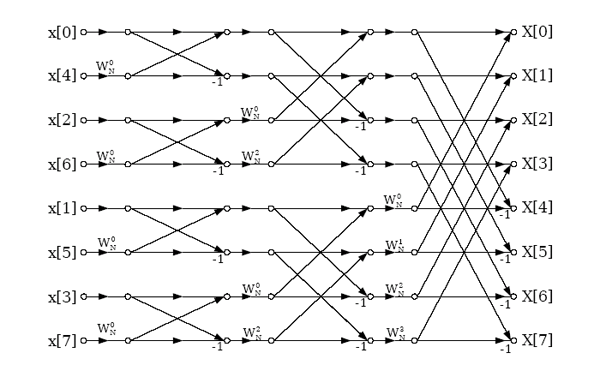
\includegraphics[width=0.6\textwidth]{butterflyRedix2}
\caption{Radix-2 8-Point FFT}
\label{Fig_Radix-2FFT}
\end{center}
\end{figure}

From the diagram, there were twice times of division of even and odd sequences. The first time division spilt the even and odd sequences. The second time, we took even and odd sequences retrieved from last division as two new sequences and split both of them into the even and odd sequences again. So far from the lowest level, we can consider our original sequence as a four-piece sequences. And then we can compute the sequence from the lowest level. Thus, we can develop our algorithm to a bigger domain. Unless the number of terms
in a sequence is in pattern of  $2^s$($s\in\mathbb{Z}$, s $<$ 20), the sequence can be reduced until the smallest piece is consist of two terms.\\
\\
Radix-2 IFFT implements the same algorithim.\\

~\newline

%Instance Model 2

\noindent
\begin{minipage}{\textwidth}
\renewcommand*{\arraystretch}{1.5}
\begin{tabular}{| p{\colAwidth} | p{\colBwidth}|}
  \hline
  \rowcolor[gray]{0.9}
  Number& IM\refstepcounter{instnum}\theinstnum \label{I_R3C}\\
  \hline
  Label& \bf Radix-3 FFT Calculation\\
  \hline
  Input& $a_n$, $b_n$, N, r\\
  &The input is constrained so that  r = 3.\\
&If invoking the real data FFT or IFFT library, there is no $b_n$ to be entered.\\
  \hline
  Output& X[k], k =(0, 1, ...,  N),  in format 'a + bi'\\
  \hline
  Description& X[k] is the power spectral density (\si{\watt\per\hertz}),\\
&a is the real number part,\\
&b is the coefficient part of complex number part.\\
&N is the size of data.\\
&r is the radix.\\
  \hline
  Sources&~\cite{Lightstone2012} \ \\
  \hline
  Ref.\ By & -\\
  \hline
\end{tabular}
\end{minipage}\\

\subsubsection*{Detailed Radix-3 FFT Algirithm}

\begin{align*}
X[k] &= \sum\limits_{n=0}^{N-1}x(n)W_{N}^{kn}\\
& = \sum\limits_{n = 3^r}x(n)W_{N}^{kn} + \sum\limits_{n = 3^r+1}x(n)W_{N}^{kn} + \sum\limits_{n = 3^r+2}x(n)W_{N}^{kn}\\
& = \sum\limits x_1(n)W_{N}^{kn} + \sum\limits x_2(n)W_{N}^{kn} + \sum\limits x_3(n)W_{N}^{kn}  ()\\
\end{align*}


Define n = 3r, n = 3r + 1 and n = 3r +2, r = 0, 1, 2, ..., N/3 -1.\\

\begin{align*}
X[k] &= \sum\limits_{r=0}^{N/3 -1}x(3r)W_{N}^{3kr} + \sum\limits_{r=0}^{N/3 -1}x(3r+1)W_{N}^{(3r+ 1)k} + \sum\limits_{r=0}^{N/3 -1}x(3r+2)W_{N}^{(3r+ 2)k}\\
& =  \sum\limits_{r=0}^{N/3 -1}x(3r)(W_{N}^{3})^{kr} + W_{N}^{k}\sum\limits_{r=0}^{N/3 -1}x(3r+1)(W_{N}^{3})^{kr} + W_{N}^{2k}\sum\limits_{r=0}^{N/3 -1}x(3r+2)(W_{N}^{3})^{kr}\\
\end{align*}

According to Eular's Formula, $W_{N}^{a}$ = $W_{N/a}$,\\

\begin{align*}
X[k] & =  \sum\limits_{r=0}^{N/3 -1}x(3r)(W_{N}^{3})^{kr} + W_{N}^{k}\sum\limits_{r=0}^{N/3 -1}x(3r+1)(W_{N}^{3})^{kr} + W_{N}^{2k}\sum\limits_{r=0}^{N/3 -1}x(3r+2)(W_{N}^{3})^{kr}\\
& = \sum\limits_{r=0}^{N/3 -1}x(3r)(W_{N/3})^{kr} + W_{N}^{k}\sum\limits_{r=0}^{N/3 -1}x(3r+1)(W_{N/3})^{kr} + W_{N}^{2k}\sum\limits_{r=0}^{N/3 -1}x(3r+2)(W_{N/3})^{kr}\\
& = X_1[k] + W_N^kX_2[k] + W_N^{2k}X_3[k]\\
\end{align*}

We can use FFT butterfly diagram to analysis a FFT computing process and we can clearly tell how the sequence is divided and computed. Here we will have a simplest
N = 9, radix-3, butterfly diagram as example:\\

Figure~\ref{Fig_Radix-3FFT}

\begin{figure}[h!]
\begin{center}
 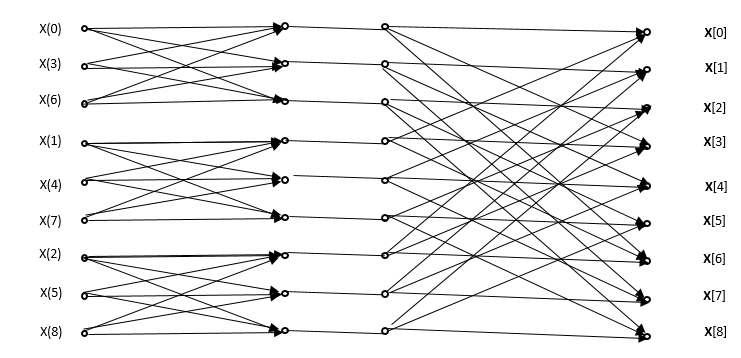
\includegraphics[width=0.6\textwidth]{butterflyRedix3}
\caption{Radix-3 9-Point FFT}
\label{Fig_Radix-3FFT}
\end{center}
\end{figure}

From the diagram, there were two times of division of sequences. Each division split sequence into three parts. The first sequence is the sum of all terms whose sequence number can be divided by 3 without the rest. The second sequence is the sum of all terms whose sequence number can be divided by 3 with rest of 1. The third sequence is the sum of all terms whose sequence number can be divided by 3 with the rest of 2. The first time division spilt the sequence into three parts following the rules as mentioned. The second time, we implement the same rule to split these three sequences so that each sequence is divided into three sequences. So far from the lowest level, we can consider our original sequence as a nine-piece sequences. And then we can compute the sequence from the lowest level. Thus, we can develop our algorithm to a bigger domain. Unless the number of terms
in a sequence is in pattern of  $3^s$($s\in\mathbb{Z}$, s $<$ 20), the sequence can be reduced until the smallest piece is consist of three terms.\\
\\
Radix-3 IFFT implements the same algorithim.\\



\section{Variabilities}

\subsection{Assumptions}

\begin{itemize}

\item[A\refstepcounter{assumpnum}\theassumpnum \label{A_N2}:]
The number of  input of radix-2 FFT and IFFT shoud be $2^s$($s\in\mathbb{Z}$, s $<$ 20) [\iref{I_R2C}, \ddref{D_OT}].
\item[A\refstepcounter{assumpnum}\theassumpnum \label{A_N3}:]
The number of input of radix-3 FFT and IFFT should be $3^s$($s\in\mathbb{Z}$, s $<$ 20) [\iref{I_R3C}].
\item[A\refstepcounter{assumpnum}\theassumpnum \label{A_Equal}:]
The length of $X[k]$ sequence is always equal to the length of sequence $x(n)$  [\tref{T_DFT}, \tref{T_IDFT}, \iref{I_R2C}, \iref{I_R3C} ].
\item[A\refstepcounter{assumpnum}\theassumpnum \label{A_CoI}:]
The coefficient of every term in $x(n)$ is an integer for both complex and real number  [\iref{I_R2C}, \iref{I_R3C}].
\item[A\refstepcounter{assumpnum}\theassumpnum \label{A_C0}:]
When retrieving the complex number FFT function, some terms are still real numbers. Users enter 0 as an coefficient for complex terms under this occation [\iref{I_R2C}, \iref{I_R3C}].
\item[A\refstepcounter{assumpnum}\theassumpnum \label{A_Stride}:]
Assume the strides for ${X}[n]$ and ${x}(n)$ are both 1 [\iref{I_R2C}, \iref{I_R3C},  \ddref{D_PSD}, \ddref{D_OT}, \ddref{D_ET}].
\item[A\refstepcounter{assumpnum}\theassumpnum \label{A_Length}:]
The length of input sequence is known [\iref{I_R2C}, \iref{I_R3C}].


\end{itemize}

\subsection{Calculation} \label{sec_Calculation}
Not Applicable. \wss{Your calculation variabilities are the choices between the
  different algorithms.}
\subsection{Output} \label{sec_Output}    
Not Applicable.



\section{Traceability Matrices and Graphs}
The purpose of the traceability matrices is to provide easy references on what has to be additionally modified if a certain component is changed.  Every time a 
component is changed, the items in the column of that component that are 
marked with an ``X'' should be modified as well.  Table~\ref{Table:trace}
shows the dependencies of theoretical models, data
definitions, and instance models with each other.
 Table~\ref{Table:A_trace} shows the dependencies of theoretical models, data definitions,  instance models, and likely changes on the assumptions.

\afterpage{
\begin{landscape}
\begin{table}[h!]
\centering
\begin{tabular}{|c|c|c|c|c|c|c|c|}
\hline
	& \aref{A_N2}& \aref{A_N3}& \aref{A_Equal}& \aref{A_CoI}& \aref{A_C0}& \aref{A_Stride}& \aref{A_Length}\\
\hline
\tref{T_DFT}   & & &X & & & & \\ \hline
\tref{T_IDFT}  & & &X & & & & \\ \hline
\tref{T_EF}   & & & & & & &  \\ \hline
\tref{T_POW}  & & X& & & &&  \\ \hline
\tref{T_TOW}  & & & & & & &  \\ \hline
\ddref{D_SRE}  & & & X& & & &\\ \hline
\ddref{D_PSD}  & & & & & &X &\\ \hline
\ddref{D_AF}   & & & & & & &  \\ \hline
\ddref{D_OT}   & X& & & & & &\\ \hline
\ddref{D_ET}    & & & & &  &X&\\ \hline
\iref{I_R2C}     & X& & X& X&X &X  &X\\ \hline
\iref{I_R3C}    & & X&X &X &X &X &X \\ \hline
\end{tabular}
\caption{Traceability Matrix Showing the Connections Between Assumptions and Other Items}
\label{Table:A_trace}
\end{table}
\end{landscape}
}

\begin{table}[h!]
\centering
\begin{tabular}{|c|c|c|c|c|c|c|c|c|c|c|c|c|}
\hline        
	& \tref{T_DFT}& \tref{T_IDFT}& \tref{T_EF}& \tref{T_POW}& \tref{T_TOW}&\ddref{D_SRE}&\ddref{D_PSD} & \ddref{D_AF}&\ddref{D_OT}&\ddref{D_ET}& \iref{I_R2C}& \iref{I_R3C} \\
\hline
\tref{T_DFT}  & & &X & & & & & & & &X &X \\ \hline
\tref{T_IDFT}  & & & & & & & & & & &X & X\\ \hline
\tref{T_EF}   & & & & X&X & & & & & &X &X \\ \hline
\tref{T_POW}  & X& & & & & & & & & &X &X \\ \hline
\tref{T_TOW}  & & & & & & & & & & &X &X \\ \hline
\ddref{D_SRE}  & & & & & & & & & & &X &X \\ \hline
\ddref{D_PSD}  & X&X & & & & & & & & &X & X\\ \hline
\ddref{D_AF}   & X& X& & & & & & & & & X&X \\ \hline
\ddref{D_OT}   & & & & & & & & & & &X& \\ \hline
\ddref{D_ET}    & & & & & & & & & & &X & \\ \hline
\iref{I_R2C}     & & & & & & & & & & & &  \\ \hline
\iref{I_R3C}    & X& & & & & & & & & & & \\ \hline

\end{tabular}
\caption{Traceability Matrix Showing the Connections Between Items of Different Sections}
\label{Table:trace}
\end{table}

The purpose of the traceability graphs is also to provide easy references on
what has to be additionally modified if a certain component is changed.  The
arrows in the graphs represent dependencies. The component at the tail of an
arrow is depended on by the component at the head of that arrow. Therefore, if a
component is changed, the components that it points to should also be
changed.\par
NOTE: Building a tool to automatically generate the graphical representation of
the matrix by scanning the labels and reference can be future work.


\newpage

\bibliographystyle {plainnat}
\bibliography {../../ReferenceMaterial/References}


\end{document}